\section*{Problem 1}
	\begin{proof} [Solution]
		My city is Yeongju which is ranked at 72 with 108,443. The below is a population distribution of all  cities in Korea based on log scale.
		\begin{center}
			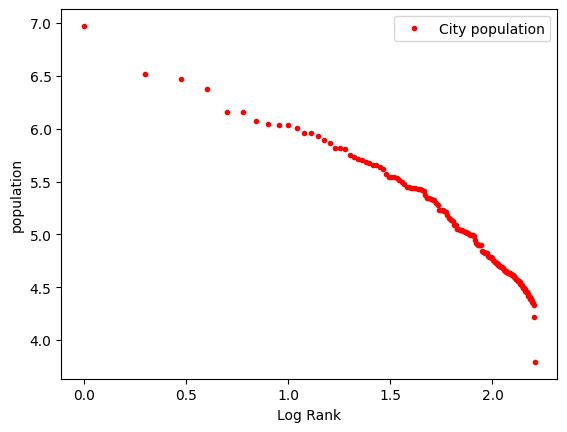
\includegraphics[width=0.5\textwidth]{pops.png}
		\end{center}
		To determine the given constants, use the linear regression to minimize the squared error.
		\begin{center}
			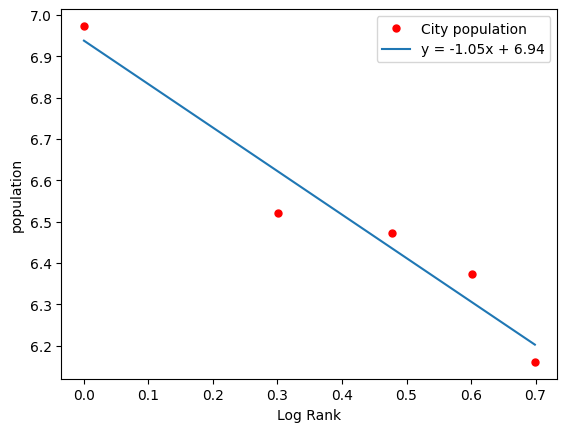
\includegraphics[width=0.5\textwidth]{pops_reg.png}
		\end{center}
		Note that I just put $C = 0$. Even though we can change $C$, it is impossible to find a value that perfectly fits the five pieces of data. By the log scale transformation, we have:
		\begin{equation*}
			\log{P(r)} = \beta \log{(r + C)} + \log{\alpha}
		\end{equation*}
		From the above line, we get
		\begin{align*}
			\beta &= -1.05\\
			\log{\alpha} &= 6.94 \Rightarrow \alpha = 10^{6.94}
		\end{align*}
		By this result, we have the relation between total cities and the line.
		\begin{center}
			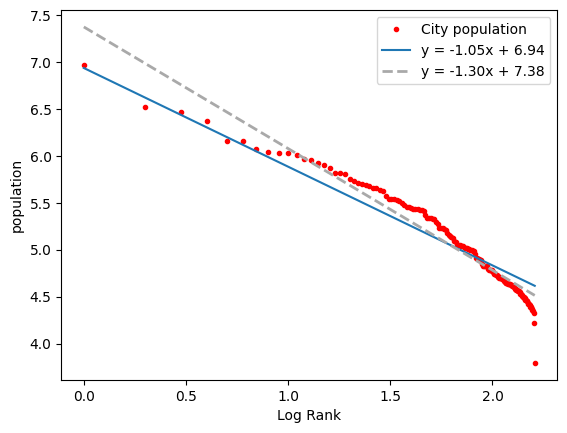
\includegraphics[width=0.5\textwidth]{pops_real.png}
		\end{center}
		The line $y = -1.30x + 7.38$ is the result of regression using all cities. They are mostly linearly distributed, but we can see that regression does not work well for some data. Clear outliers at both ends prevent Zipf\textquotesingle s law from working. Still, excluding these things, urban distribution can be explained as almost following Zipf\textquotesingle s law. There are a variety of variables that may be involved in this alignment. If there is a primate city, like Seoul, it can deviate from this rule depending on how much control it has. There may be significant differences in population depending on the level of economic and industrial growth in the region. In the case of Ulleung-gun, which is ranked last, it can be seen that the population is extremely low due to the geographical feature of being a city made up of very small islands.\\
	\end{proof}